% {Youssouph Cissokho}

\section{Applications à des problèmes réels}\label{Section:6}

Dans cette section, nous fournirons une comparaison expérimentale de quelques méthodes classiques  mentionnées ci-haut  pour tester et comparer les techniques de détection des valeurs aberrantes proposées sur des données réelles.
\noindent\textbf{Prétraitement des données} Tous les ensembles de données ont été normalisés pour que ceux qui ont une grande échelle ne dominent pas les autres et les variables qualitatives ont été enlevèes avant de les passer aux algorithmes.

\noindent Certains algorithmes mentioné dans la section \ref{Section:2} sont considérés dans cette étude tel que \textbf{Local Outlier Factor (LOF), Isolation Forest, $k$ Nearest Neighbours and Analyse des composantes principales (ACP)}. Les paramètres par défaut sont utilisés pour toutes les méthodes. Le code en python peut être trouvé dans l'annexe de ce rapport. \newl



%
% data set 1
%
\noindent \textbf{a) Jeu de données 1: Compagnies aériennes:} Comprend les informations sur tous les vols intérieurs aux USA  en 2019, tels que l'heure de départ, l'heure d'arrivée, l'aéroport d'origine, l'aéroport de destination, etc. disponible  \href{https://www.transtats.bts.gov/DL_SelectFields.asp?Table_ID=}{\textcolor{blue}{\underline{ici}}}. Il est question d’analyser les retards accusés aux  départs et/ou à l’arrivée des vols. En effet, un vol est considéré comme à “l’heure”  \textbf{s’il arrive moins de 15 minutes plus tard que l'heure indiquée} dans les systèmes de réservation informatisés (CRS) du transporteur. Par conséquent, les \textbf{anomalies sont des vols avec des retards chroniques}. Pour ce faire, un échantillon de $10000$ de vols qui prennent départ au niveau de l'aéroport O'Hare de Chicago (ORD) est extrait et les temps de retard moyens sont calculés par rapport aux temps d'arrivée à l'aéroport. Le temps d'arrivée moyen est calculé pour tous les vols atterrissant à un aéroport donné.\textbf{Les anomalies sont des vols avec des retards chroniques (plus de 15 minutes) ( c'est-à-dire la différence en minutes entre l'heure d'arrivée prévue et l'heure d'arrivée réelle).} Cependant, le \textb{nombre négatif indiquent que le vol est arrivé plus tôt que l'heure prévue, ses vols ne sont donc pas considérés comme des arrivées tardives}.  L'objectif est d'analyser les retards dans les heures d'arrivée pour chaque vol.
\begin{figure}[H]
    \centering
    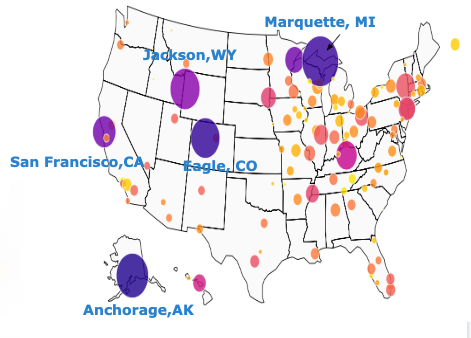
\includegraphics[width=.50\textwidth]{ADOA/Images/Vol_scatterplot.png}
    \caption{Nuage de points des retards accusés à l'arrivée avec comme taille des boules la variable ARR\_DELAY.}%\hrule
    \label{fig20}.
\end{figure}
\noindent Dans la figure \ref{fig20}, On peut facilement remarquer que les aéroports \textbf{Marquette, anchorage, Jackson et Eagle} qui présentent des retards moyens inhabituels (très élevés) et sont donc susceptibles d'avoir un comportement anormal. L'application des méthodes permettra d'identifier ces aéroports, les résultats sont présentés dans la figure \ref{fig21}.\newl
\begin{figure*}[ht]
    \centering
     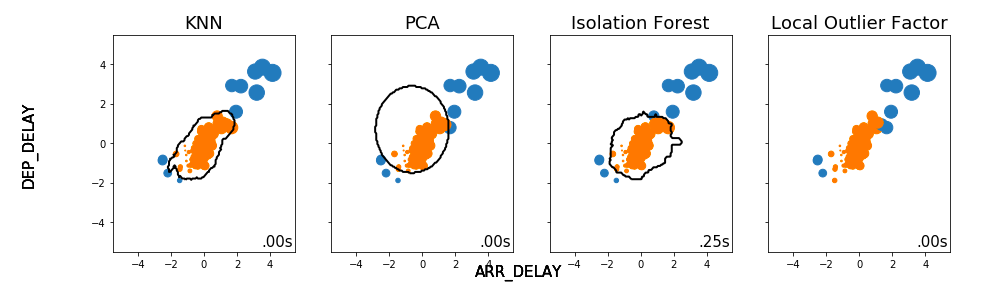
\includegraphics[width=1\textwidth]{ADOA/Images/Vol_results.png}\label{fig02}.
    \caption{Aéroports détectés comme aberrants par PCA, KNN, Isolation Forest et LOF.}%\hrule
    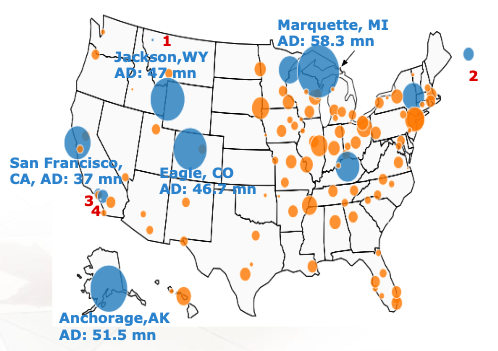
\includegraphics[width=.45\textwidth]{ADOA/Images/Vol_PCA.png}
    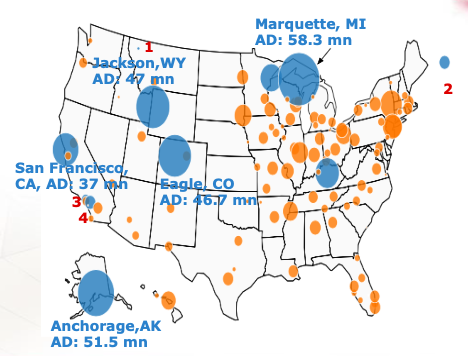
\includegraphics[width=.450\textwidth]{ADOA/Images/Vol_KNN.png}\\
    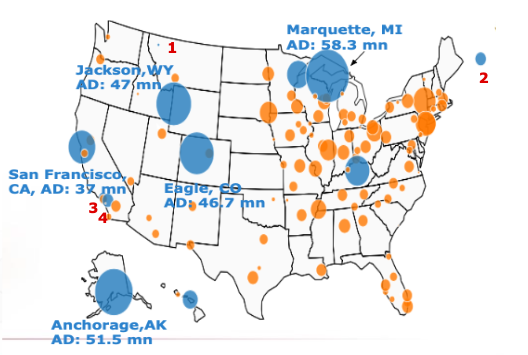
\includegraphics[width=.45\textwidth]{ADOA/Images/Vol_IsoForest.png}
    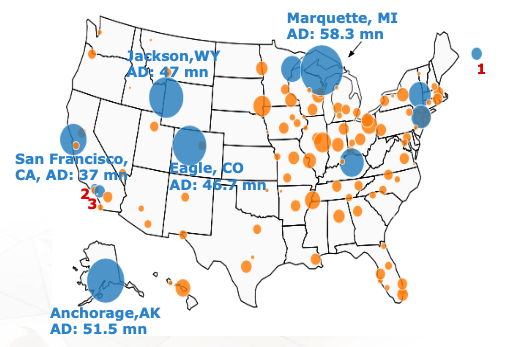
\includegraphics[width=.450\textwidth]{ADOA/Images/Vol_LOF.png}
    \caption{Aéroports détectés comme aberrants par PCA (en haut à gauche), KNN (en haut à droite), Isolation Forest (en bas à gauche) et LOF (en bas à droite)}%\hrule
    \label{fig21}
\end{figure*}

\noindent\textbf{Analyse des résultats:} 
Rappelons que les anomalies sont des vols dont le temps moyen d'arrivée est supérieur à 15 minutes. Les cercles oranges représentent les aéroports sans comportement anormal, tandis que les cercles bleus représentent les aéroports avec un comportement anormal et la taille des boules indique en moyenne, les retards à l'arrivée. En outre, dans la figure \ref{fig21}, certains aéroports sont identifiés comme aberrants par toutes les méthodes : \textbf{Eagle, San Francisco, Marquette, Anchorage}, entre autres. Cependant, des retards chroniques se sont produits à Marquette (avec 58 minutes de retard en moyenne) prèsque une heure de retard, à Anchorage (avec 51 minutes), à Jackson et Eagle ( ~ 47 minutes). Les vols qui sont arrivés plus tôt que l'heure prévue sont indiqués par des nombres négatifs, mais ils sont identifiés comme aberrants par presque toutes les méthodes :\textb{1: Kalispell (-4 minutes), 2: Oakland (-15 minutes), 3: Burbank (-12 minutes), 4: Ontario (-15 minutes)}, en d'autres termes, ils sont arrivés en moyenne 4, 15 , 12 et 15 minutes plus tôt que l'heure prévue mais ils sont faussement classés comme aberrants. Seul \textbf{Kalispell} n'est pas classé comme tel par le LOF. 
\begin{table}[t!]
\centering
 \begin{tabular}{||c c c c c||} 
 \hline
 &  KNN & PCA & IsolForest & LOF\\ [0.5ex] 
 \hline\hline
San Francisco & $\checkmark$ & $\checkmark$  & $\checkmark$ & $\checkmark$ \\ 
 Eagle & $\checkmark$ & $\checkmark$  & $\checkmark$ & $\checkmark$ \\
Marquette & $\checkmark$ & $\checkmark$  & $\checkmark$ & $\checkmark$ \\
 Kalispell & $\checkmark$ & $\checkmark$  & $\checkmark$ & $\times$ \\ [1ex] 
 \hline
 \end{tabular}
 \caption{Résumé des résultats.}
 \label{fig2w}
\end{table}

\afterpage{\FloatBarrier}

%
% data set 2
%

\noindent\textbf{b) Jeu de données 2: Accidents mortels:}
 est une donnèe qui représente les accidents mortels concernent uniquement les occupants de voitures de tourisme et de camionnettes aux États-Unis. Ces accidents impliquent toute activité susceptible de détourner l'attention d'une personne de la tâche principale de la conduite, comme envoyer des SMS, utiliser un téléphone portable, manger et boire, se toiletter, utiliser un système de navigation, régler la radio, etc. disponible  \href{https://www.bts.dot.gov/content/passenger-car-and-light-truck-occupants-killed-and-restraint-use}{\textcolor{blue}{\underline{ici}}}. \newl
\noindent\textbf{Analyse des résultats:}
Une analyse visuelle de la Figure \ref{fig2}, montre qu'il y a des pays qui se distinguent des autres avec un nombre élevé d'accidents mortels dans ces pays. D'autre part, la boîte à moustaches, nous indique également que ces pays sont anormaux (aberrants), ces pays sont \textbf{Texas, california, Florida}. Une analyse plus approfondie est menée pour corroborer les résultats antérieurs. Ces méthodes sont \textbf{ KNN, PCA, LOF and Isolation Forest}. Le resultat est présenté dans la Figure  \ref{fig2b}. 
\begin{figure}[H]
    \centering
    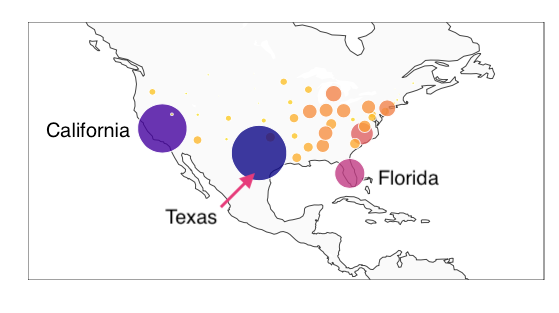
\includegraphics[width=.5\textwidth]{ADOA/Images/fat1png.png}
    \caption{Nuage de points des accidents mortels sur la carte avec comme taille des boules la variable Restraint\_used\_Fatalities}%\hrule
    \label{fig2}
\end{figure}

 \begin{figure*}[H]
    \centering
    %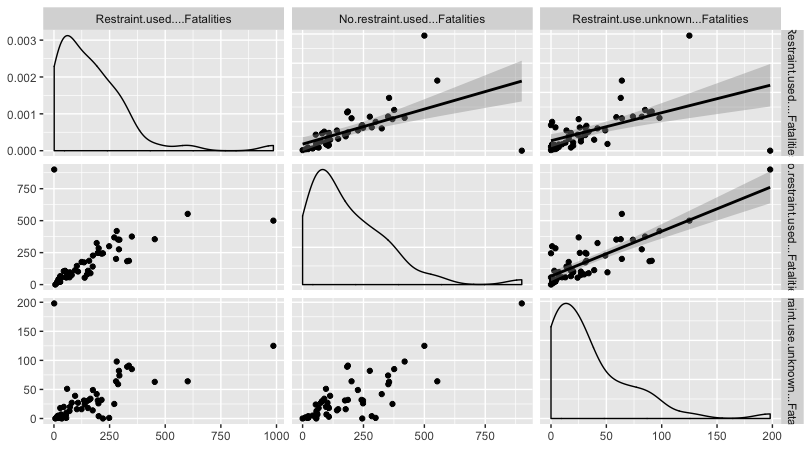
\includegraphics[width=.55\textwidth]{ADOA/Images/Fatal.png}
    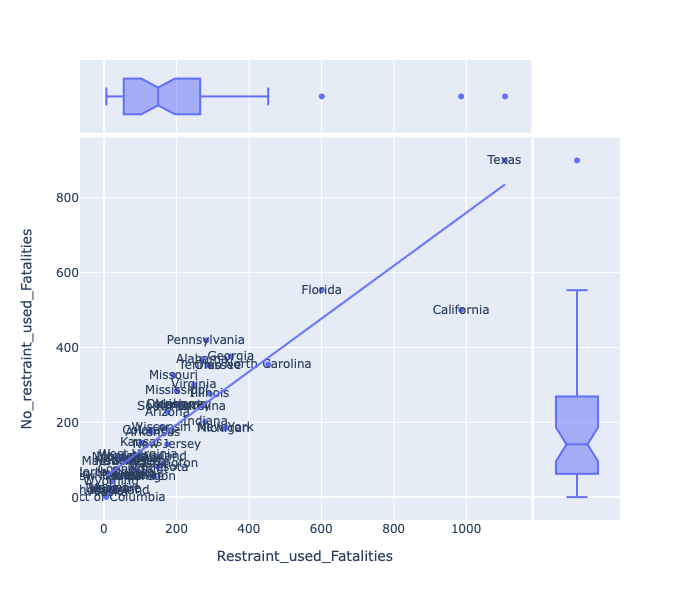
\includegraphics[width=.50\textwidth]{ADOA/Images/Fatal1.png}
    \caption{Nuage de points des accidents mortels}%\hrule
    \label{fig2a}
\end{figure*}

 \begin{figure*}[ht]
    \centering
    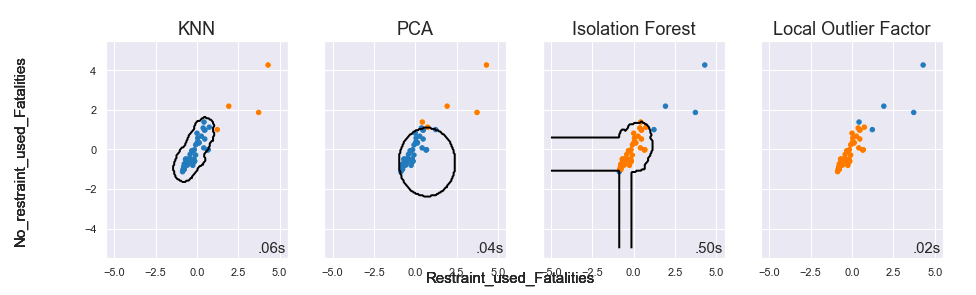
\includegraphics[width=1\textwidth]{ADOA/Images/Fatal11.png}
    \caption{Illustration des performences des méthodes: KNN, PCA, Isolation forest and LOF}%\hrule
    \label{fig3}
\end{figure*}
\vspace{2cm}

\begin{figure*}[ht]
    \centering
    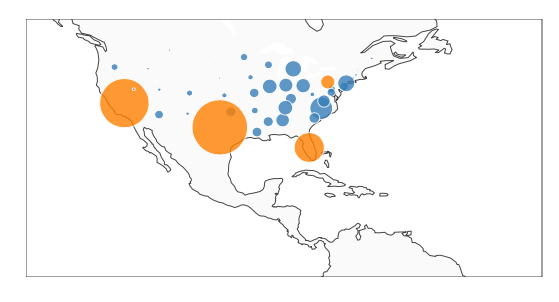
\includegraphics[width=.45\textwidth]{ADOA/Images/FatPCA.png}
    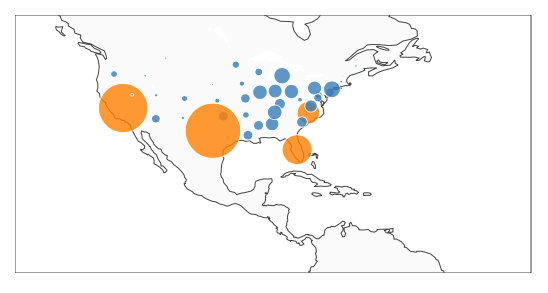
\includegraphics[width=.450\textwidth]{ADOA/Images/FatKNN.png}\\
    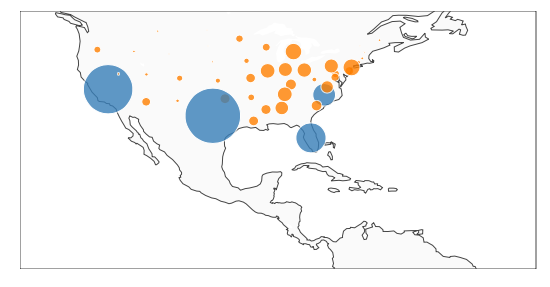
\includegraphics[width=.45\textwidth]{ADOA/Images/FatIsofore.png}
    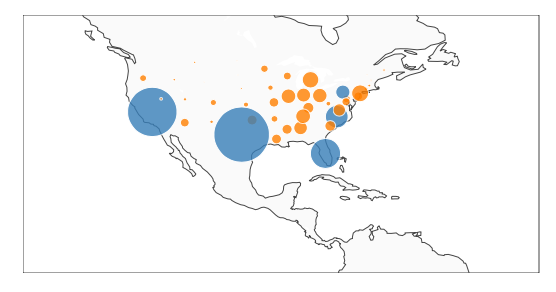
\includegraphics[width=.450\textwidth]{ADOA/Images/FatLOF.png}
    \caption{Villes qui ont plus d'accidents mortels détectées comme aberrantes par PCA (en haut à gauche), KNN (en haut à droite), Isolation Forest (en bas à gauche) et LOF (en bas à droite)}%\hrule
    \label{fig2b}
\end{figure*}

En fait, les pays \textbf{Texas, californie, Floride} sont globalement considérés comme des valeurs aberrantes (nombre élevé de décès) par la plupart des méthodes. 


%
%
\begin{table}[ht!]
\centering
 \begin{tabular}{||c c c c c||} 
 \hline
 &  KNN & PCA & IsolForest & LOF\\ [0.5ex] 
 \hline\hline
Texas & $\checkmark$ & $\checkmark$  & $\checkmark$ & $\checkmark$ \\ 
 California & $\checkmark$ & $\checkmark$  & $\checkmark$ & $\checkmark$ \\
Florida & $\checkmark$ & $\checkmark$  & $\checkmark$ & $\checkmark$ \\
 North Carolina & $\checkmark$ & $\times$  & $\times$ & $\times$ \\ [1ex] 
 \hline
 \end{tabular}
 \caption{Résumé des résultats.}
\end{table}

%
%
%
\noindent\textbf{c) Jeu de données 3: Températures en Australie:}
Cet ensemble de données décrit les températures minimales quotidiennes sur 10 ans (1981-1990) dans la ville de Melbourne, en Australie, voir Figure \ref{fig2t}. Les unités sont en degrés Celsius et il y a $3650$ observations. La source des données est attribuée au Bureau australien de météorologie et peut être téléchargé \href{https://machinelearningmastery.com/time-series-data-visualization-with-python/}{\textcolor{blue}{\underline{ici}}}. Un grand nombre d'applications génèrent des ensembles de données temporelles. Par exemple, dans notre quotidien vie, divers types de dossiers comme le crédit, le personnel, les finances, la justice, la médecine, etc., sont tous temporels. Cela souligne la nécessité d'une étude organisée et détaillée des valeurs aberrantes par rapport à ces données temporelles \cite{A5}. Les anomalies dans les séries de données  sont à l'origine des pointes inattendues, des baisses, des changements de tendance ou encore des changements de niveau. Pour une série univariée, le problème peut être considéré comme supervisé ou non. Dans le premier, deux limites son calculées (borne supérieure et inférieure), toutes les observations au delà de ces limites sont considérées comme anormales. Dane l'exemple qui suit, la méthode non supervisée est considérée. \newl
\noindent\textbf{Analyse des résultats:} 
La Figure \eqref{fig2t1} montre les résultats de quatre méthodes \textbf{PCA, IsolationForest, LOF and KNN} sur cette donnée ( à noté que La couleur bleue signifie \textbf{anormale} et \textbf{normale} pour la couleur orange). Les données sont normalisées en amont. \textbf{KNN} donne un meilleur résultat par rapport aux autres. Il parvient à detecter les températures \textbf{hautes et basses}. Cependant, les autres méthodes en détectent quelques unes mais elles génèrent beaucoup d'erreurs. \textbf{LOF}, malgré sa popularité, donne un résultat complètement erroné sur ces données. 

\begin{figure}[H]
    \centering
    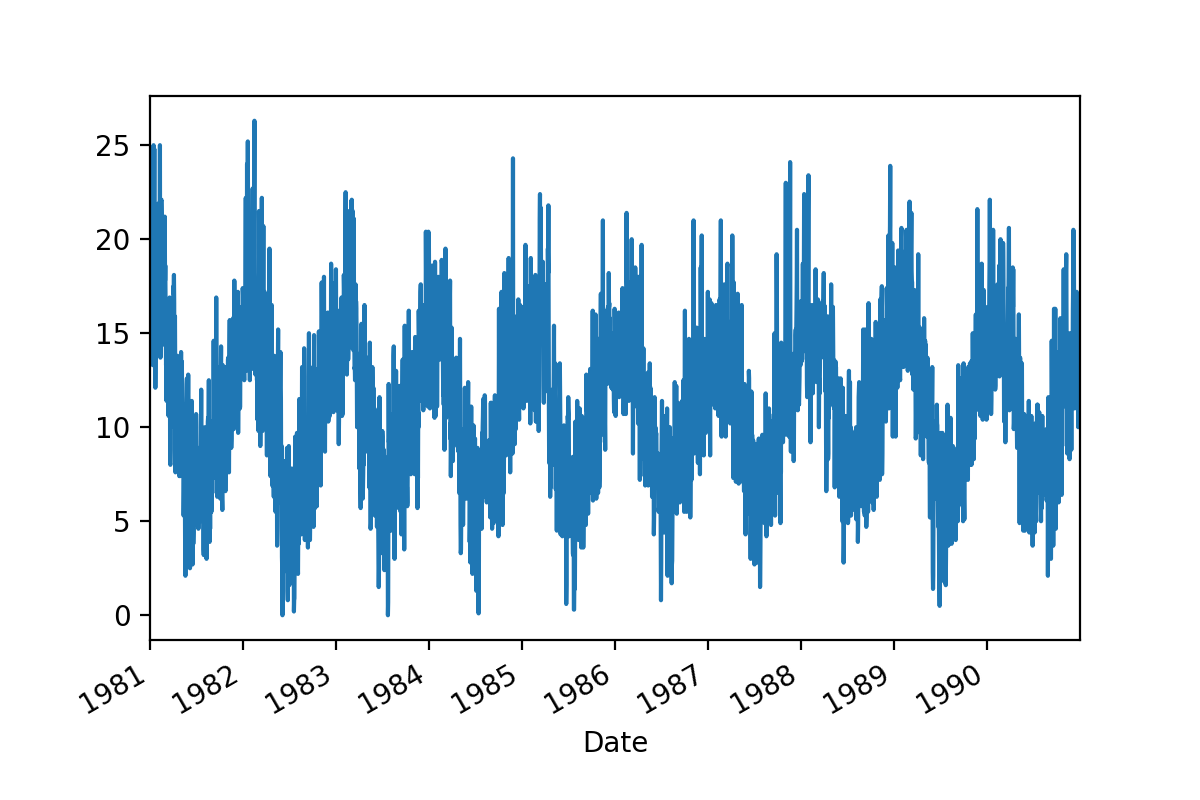
\includegraphics[width=.5\textwidth]{ADOA/Images/Temp1.png}
    %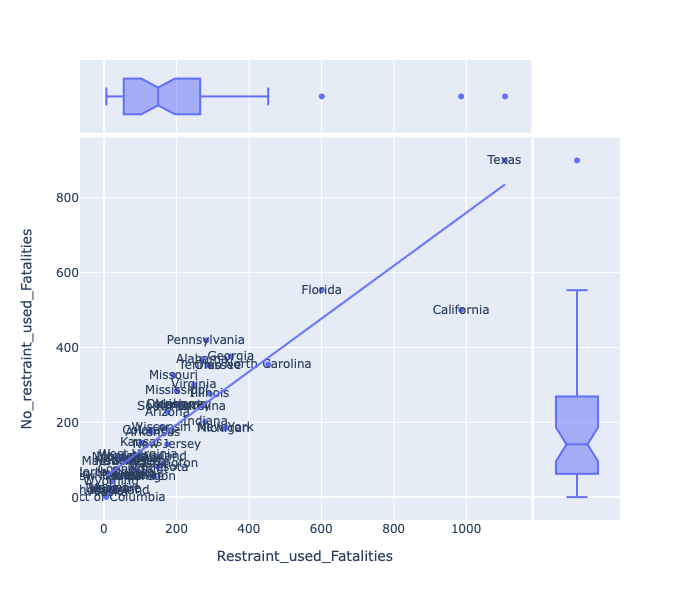
\includegraphics[width=.40\textwidth]{ADOA/Images/Fatal1.png}
    \caption{Températures minimales quotidiennes de la ville de Melbourne, en Australie (1981-1990)}%\hrule
    \label{fig2t}
\end{figure}

\begin{figure*}[ht!]
    \centering
    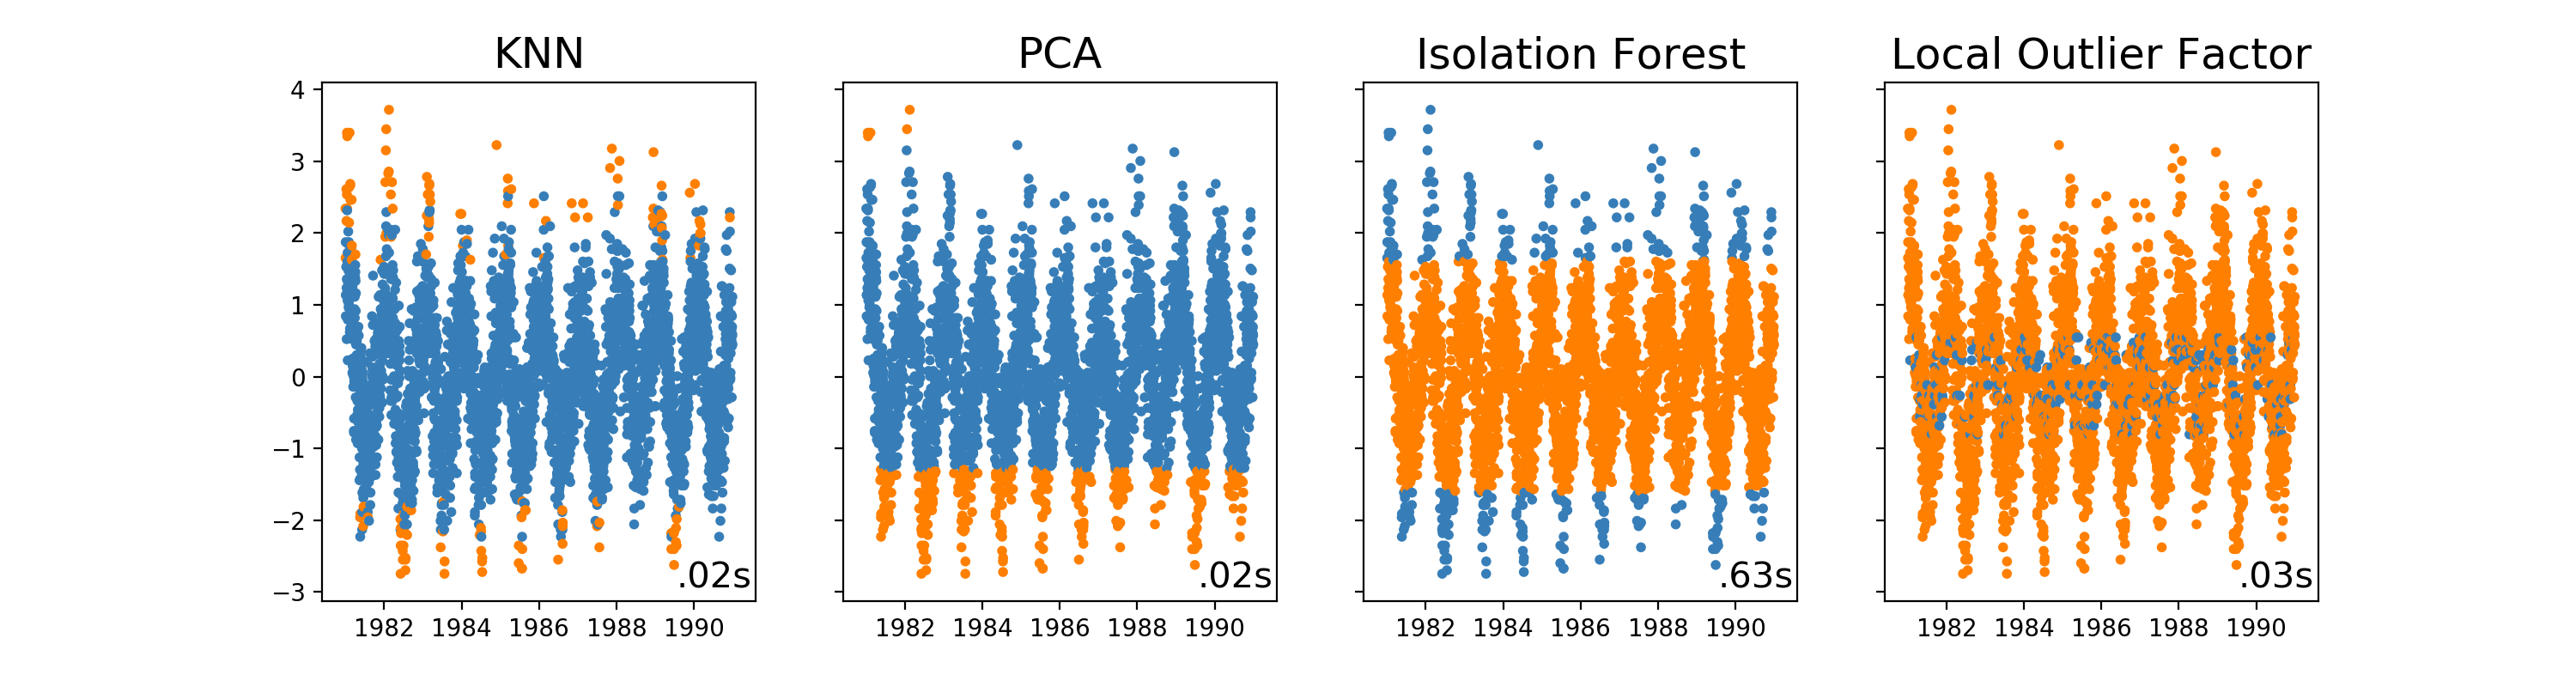
\includegraphics[width=1\textwidth]{ADOA/Images/Temp2.png}
    \caption{Températures détectées comme aberrantes par PCA, KNN, Isolation Forest et LOF.}%\hrule
    \label{fig2t1}
\end{figure*}

%
%
%
\noindent \textbf{e) Jeu de données 4: transactions :} cet ensemble de données contient des informations concernant les ventes et les produits de \textbf{salespersonnel} d'une certaine société. Les vendeurs fixent leurs propres prix de vente et rapportent les ventes à l'entreprise à la fin de chaque mois. Un faible pourcentage de ces enregistrements a été vérifié et étiqueté comme \textbf{"ok" ou "fraud"}. Il s'agit de transactions de $387010$, avec 5 variables. Après le prétraitement et l'élimination des valeurs manquantes, les observations de $15546$ sont conservées pour une analyse plus approfondie, avec $1199$ transactions frauduleuses, soit $7 \%$. Il s'agit d'un problème d'apprentissage supervisé, l'objectif est d'entrainer le modèle à identifier correctement les transactions frauduleuses et non frauduleuses et de prédire le résultat pour les transactions restantes. Les données sont disponibles dans le package "DMwR" dans R.  

Pour évaluer la performance des modèle, ces quantités sont prises en compte : \textbf{
Sensibilité, Rappel, ou taux de vrais positifs ; Spécificité ou taux de vrais négatifs ; Précision ou valeur prédictive positive ; Valeur prédictive négative ; Taux de faux positifs ; Taux de faux négatifs ; Taux de fausse découverte ; Accuracy}, voir le tableau \ref{fig_sale3}.

\noindent\textbf{Analyse des résultats:} Dans le tableau \eqref{fig_sale3}, on peut facilement voir que \textit{Isolation Forest (accuracy 91 $\%$)} et \textit{Local Outlier Factor (accuracy 87 $\%$)} surpassent \textit{KNN (accuracy 91 $\%$)} et \textit{PCA (accuracy 91 $\%$)}.

En outre, la courbe ROC \footnote{ROC (de l’anglais receiver operating characteristic, pour « caractéristique de fonctionnement du récepteur ») dite aussi caractéristique de performance (d'un test) ou courbe sensibilité/spécificité, est une mesure de la performance d'un classificateur binaire. Graphiquement, on représente souvent la mesure ROC sous la forme d'une courbe qui donne le taux de vrais positifs (fraction des positifs qui sont effectivement détectés) en fonction du taux de faux positifs (fraction des négatifs qui sont incorrectement détectés).} et l'\textbf{Aire sous la courbe ROC ou (AUC)}\footnote{c'est un outil \textbf{visuel} pour mesurer la performence  des modèles et de les comparer. Un test \textbf{parfait} correspond à une aire de $1$ tandis qu'un test \textbf{mauvais} correspond à une aire de $0,5$. Un guide pour la classification est donné par le système de points: \textbf{
.90-1 = \textcolor{blue}{très bon (A)} ; .80-.90 = \textcolor{blue}{bon (B)}; .70-.80 = \textcolor{blue}{raisonnable (C)}; .60-.70 = \textcolor{blue}{faible (D)} et .50-.60 = \textcolor{blue}{échoué (F)}}\cite{ROC}} (Figure \ref{fig_sal14}
sont des méthodes visuels de discrimination entre les algorithmes. En effet, d'après le graphique, \textbf{Isolation Forest} est un \textbf{bon} modèle pour cet ensemble de données avec un AUC de $0.870$, suivi de LOF avec un AUC de $0.632$. \noindent Cependant, PCA (AUC =$.56$) et KNN (AUC=$.23$) donnent un mauvais résultat. Figure \ref{fig_sal13} donne la matrice de confusion de Isolation Forest. Parmi $1119$ transactions frauduleuses, il identifie correctement $521$ i.e. un taux de $ 43 \%$ de VP et $678$ comme des transactions normales, soit un taux de $ 57 \%$ de  FN. De même, parmi $15546$ transactions normales, il trouve $13671$ comme tel, soit un taux de $95 \%$ de VN  et $676$ comme frauduleuses,  soit un taux de $5 \%$ de FP. 
\begin{table}[H]
\centering
 \begin{tabular}{||l c c c c||} 
 \hline
 &  KNN & PCA & IsolForest & LOF\\ [0.5ex] 
 \hline\hline
Rappel & 4 \% & 7 \%  & 95 \% & 93  \% \\ 
Spécificité & 67 \% & 86 \%  & 43 \% & 18 \% \\
Précision & 58 \% & 86 \%  & 95 \% & 93 \% \\
VPN & 6 \% & 7 \%  & 44 \% & 18 \% \\
FP & 34 \% & 14 \%  & 57 \% & 82 \% \\
FN & 96 \% & 93 \%  & 5 \% & 7 \% \\
FD & 42 \% & 14 \%  & 5 \% & 7 \% \\
Accuracy & 9 \% & 13 \%  & \textcolor{blue}{91} \% & \textcolor{blue}{87} \% \\
[1ex] 
 \hline
 \end{tabular}
 \caption{Résumé des résultats de l'ensemble de données sur les opérations de vente.}
 \label{fig_sale3}
\end{table}
%\end{figure*}

\begin{figure}[H]
    \centering
    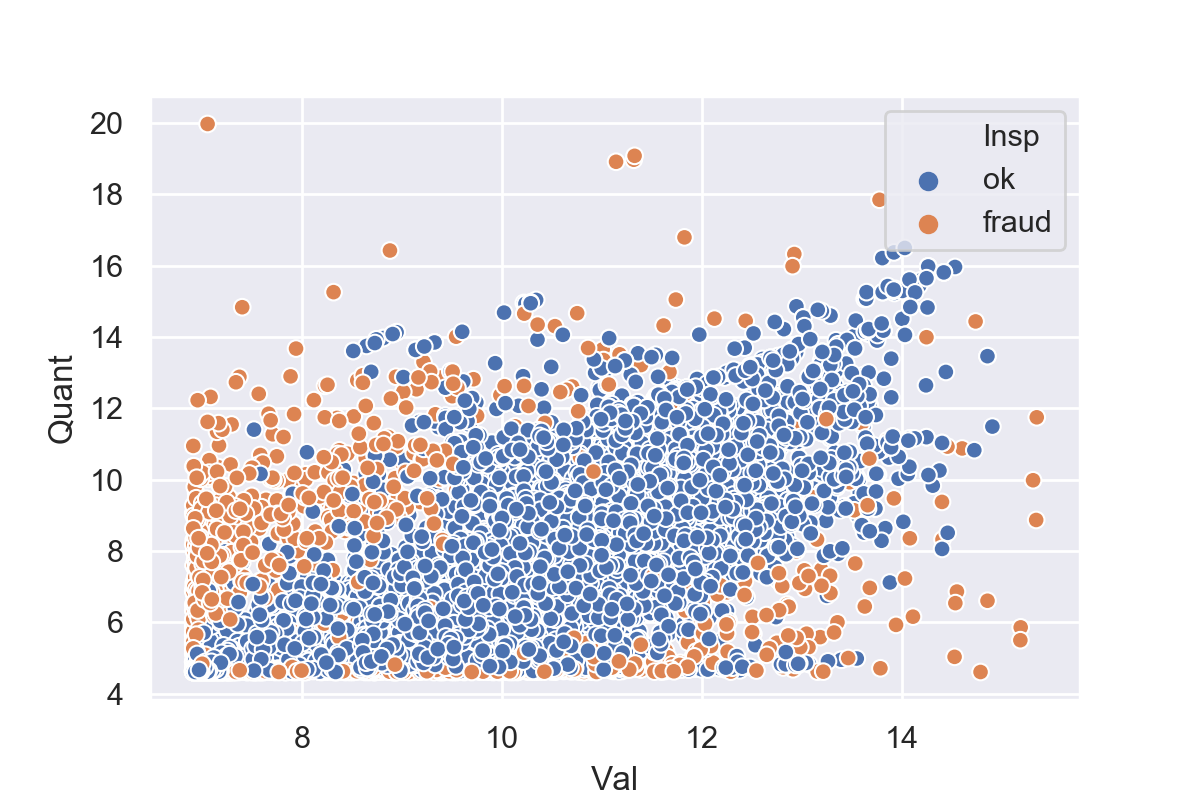
\includegraphics[width=.5\textwidth]{ADOA/Images/salescatter.png}
    \label{fig_sal11}
    \caption{Nuage de points des transactions.}%\hrule
\end{figure}

% roc and conusion matrix
\begin{figure}[H]
    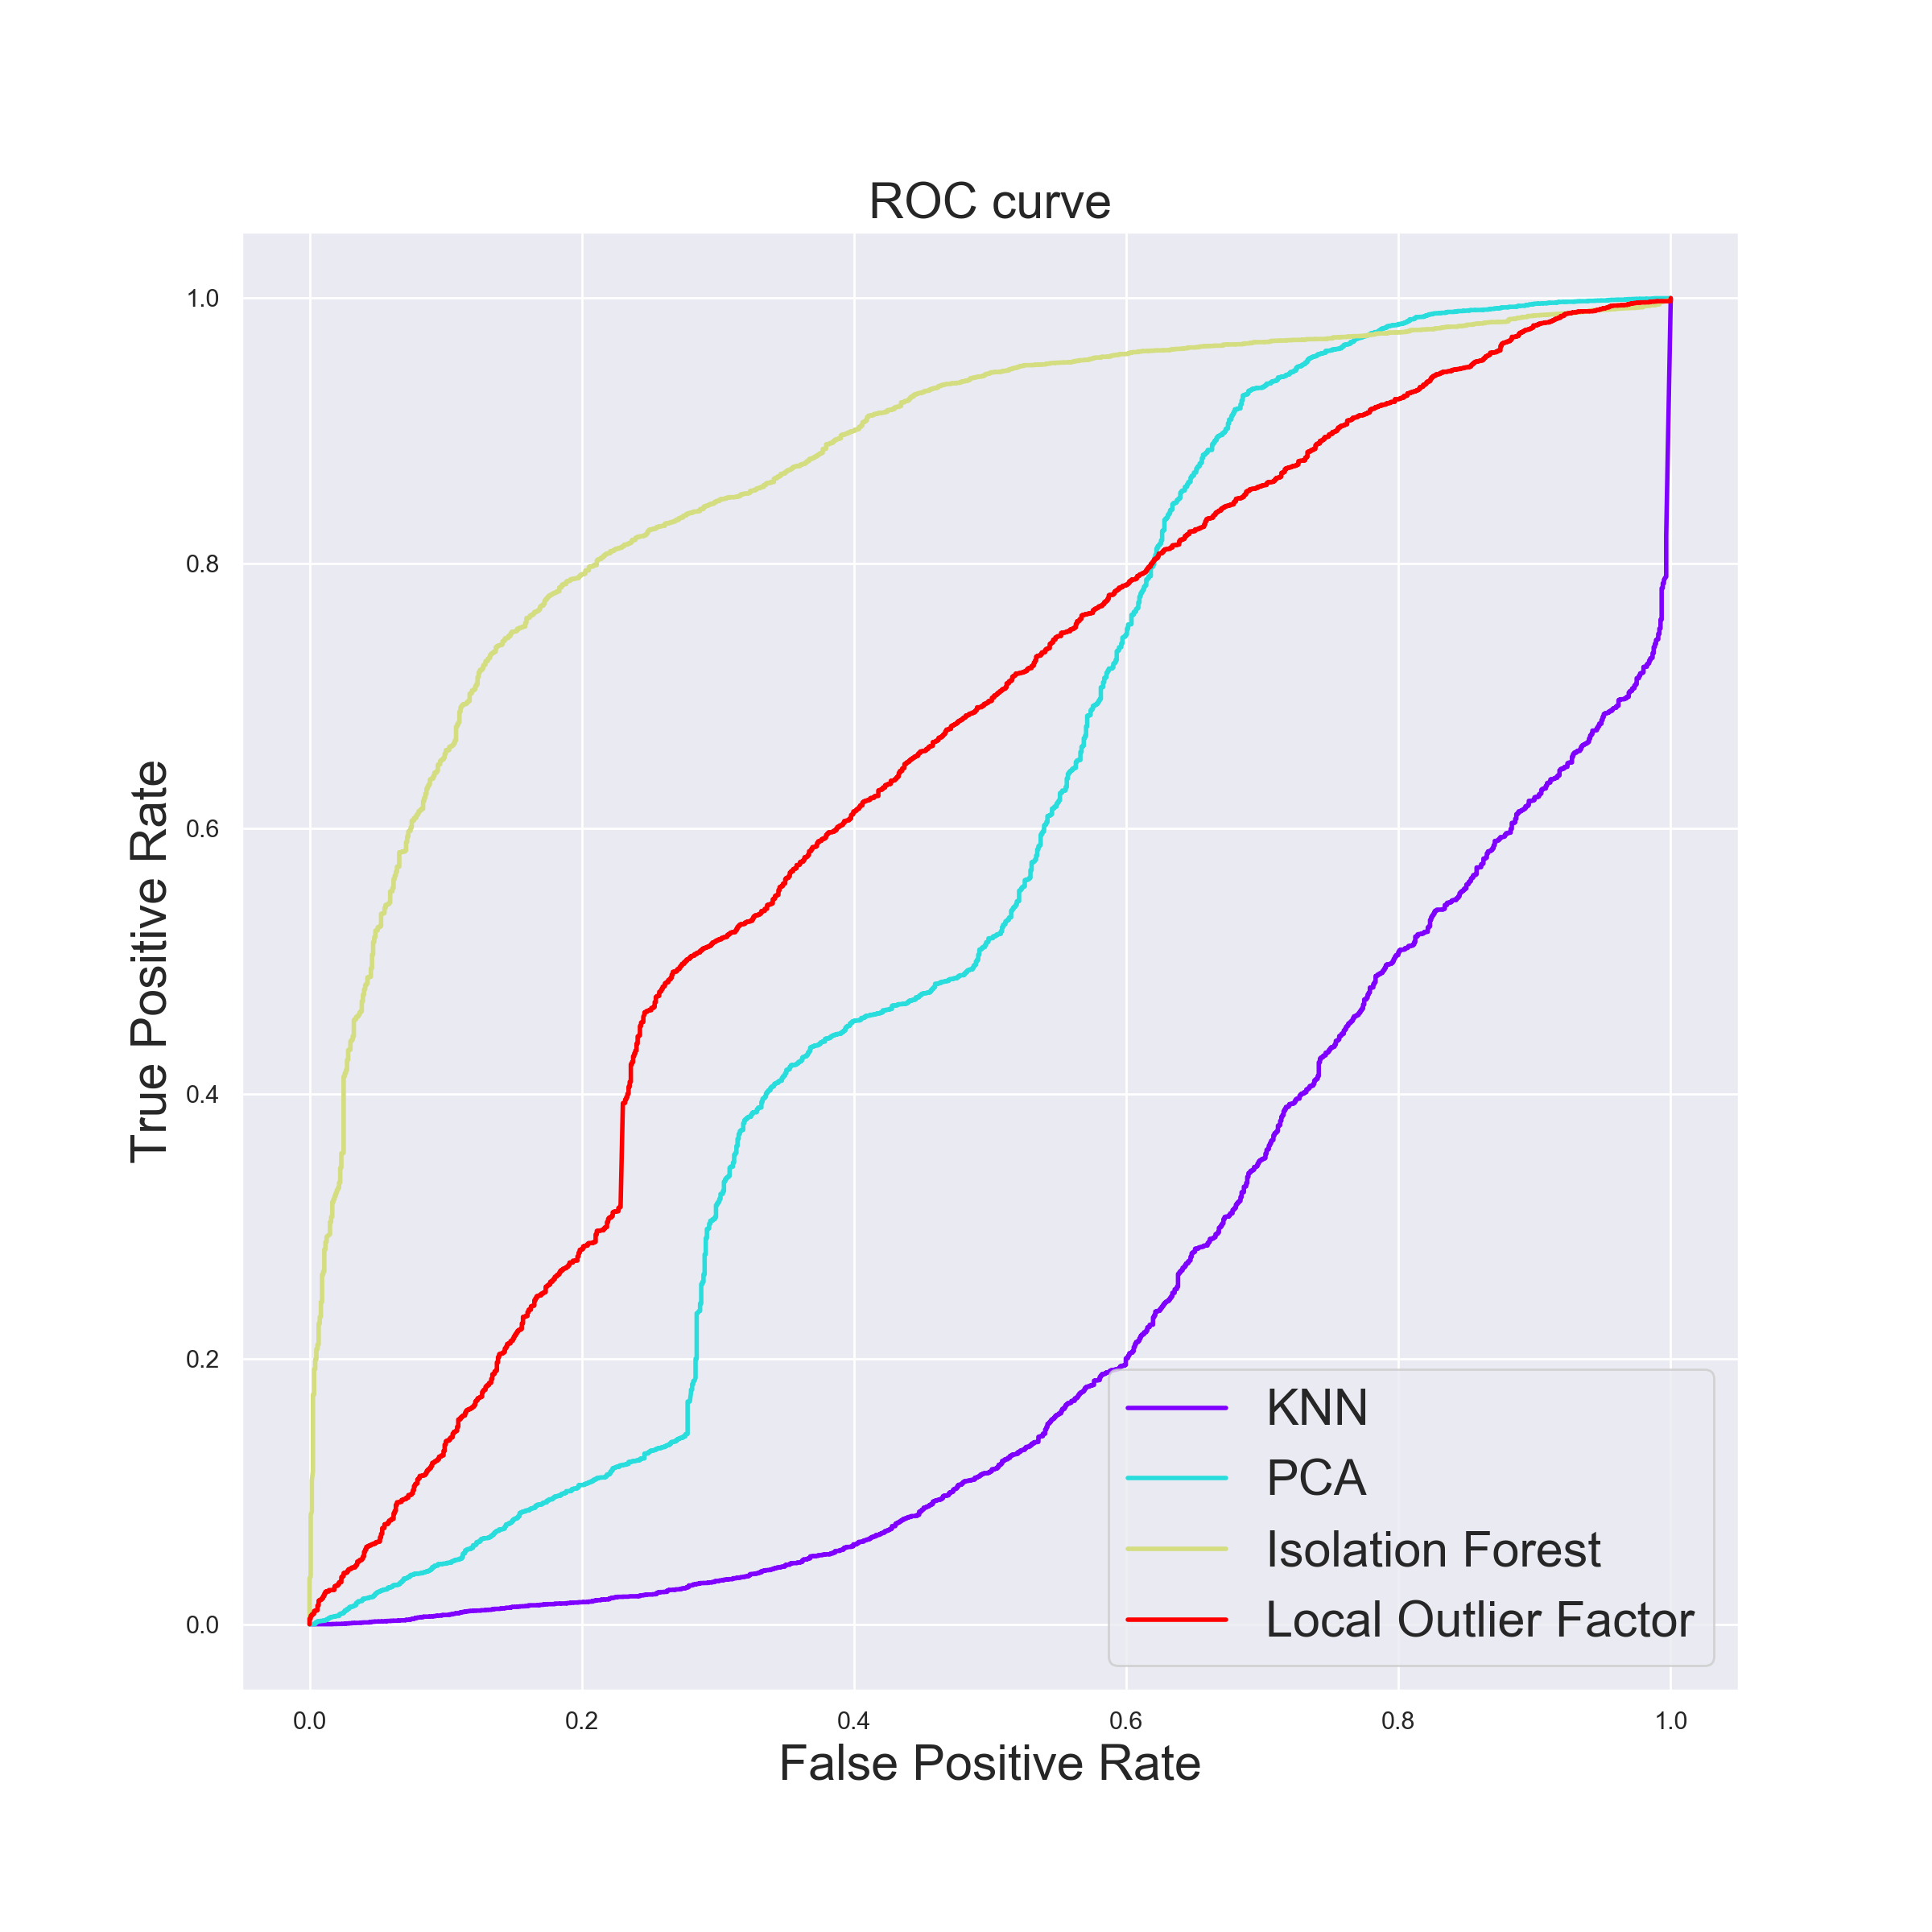
\includegraphics[width=.4\textwidth]{ADOA/Images/sales_roc.png}
     \caption{Courbe ROC pour PCA, KNN, Isolation Forest, LOF.}%\hrul
     \label{fig_sal14}
    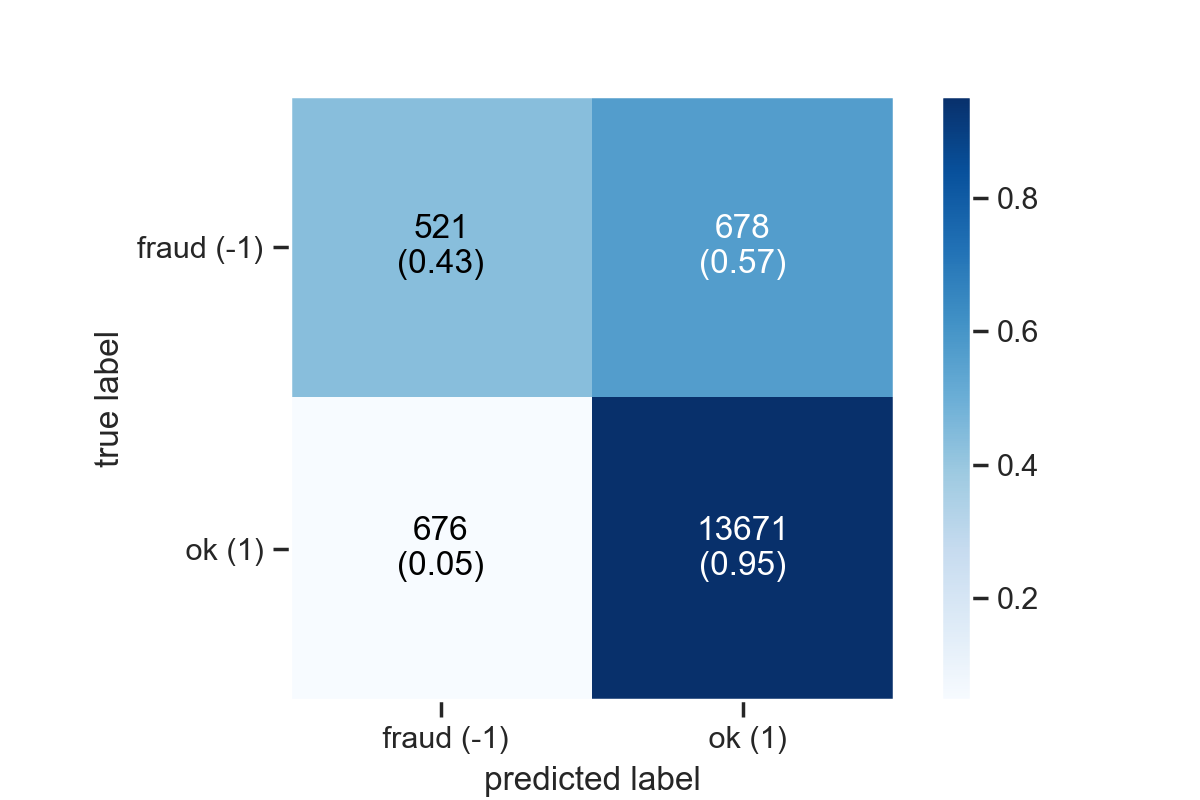
\includegraphics[width=.5\textwidth]{ADOA/Images/sales_confusionmat.png}
  \caption{Matrice de confusion pour Isolation Forest.}
    \label{fig_sal13}
\end{figure}

% boxplot
\begin{figure}[H]
    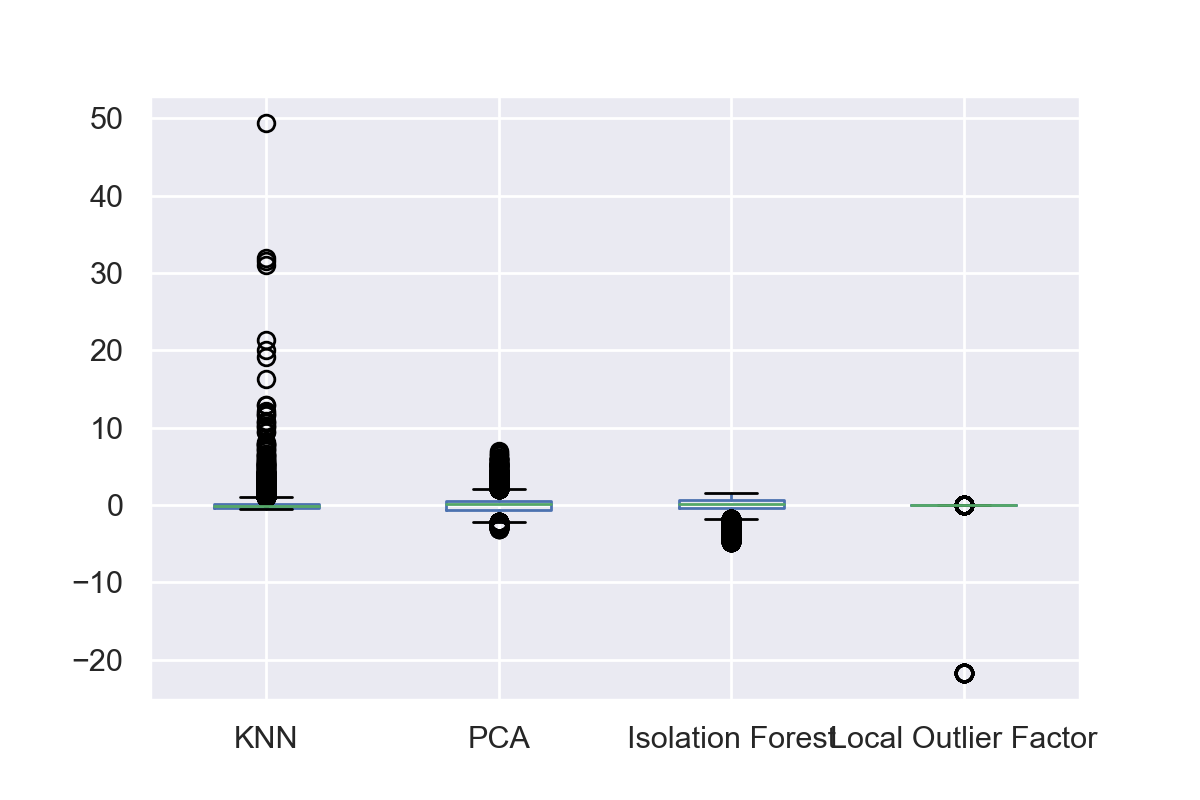
\includegraphics[width=.45\textwidth]{ADOA/Images/sales_boxplot.png}
    \label{fig_sal12}
    \caption{Boîte à moustaches pour PCA, KNN, Isolation Forest, LOF.}%\hrule
\end{figure}

% resultats des methodes
\begin{figure*}[ht!]
    \centering
    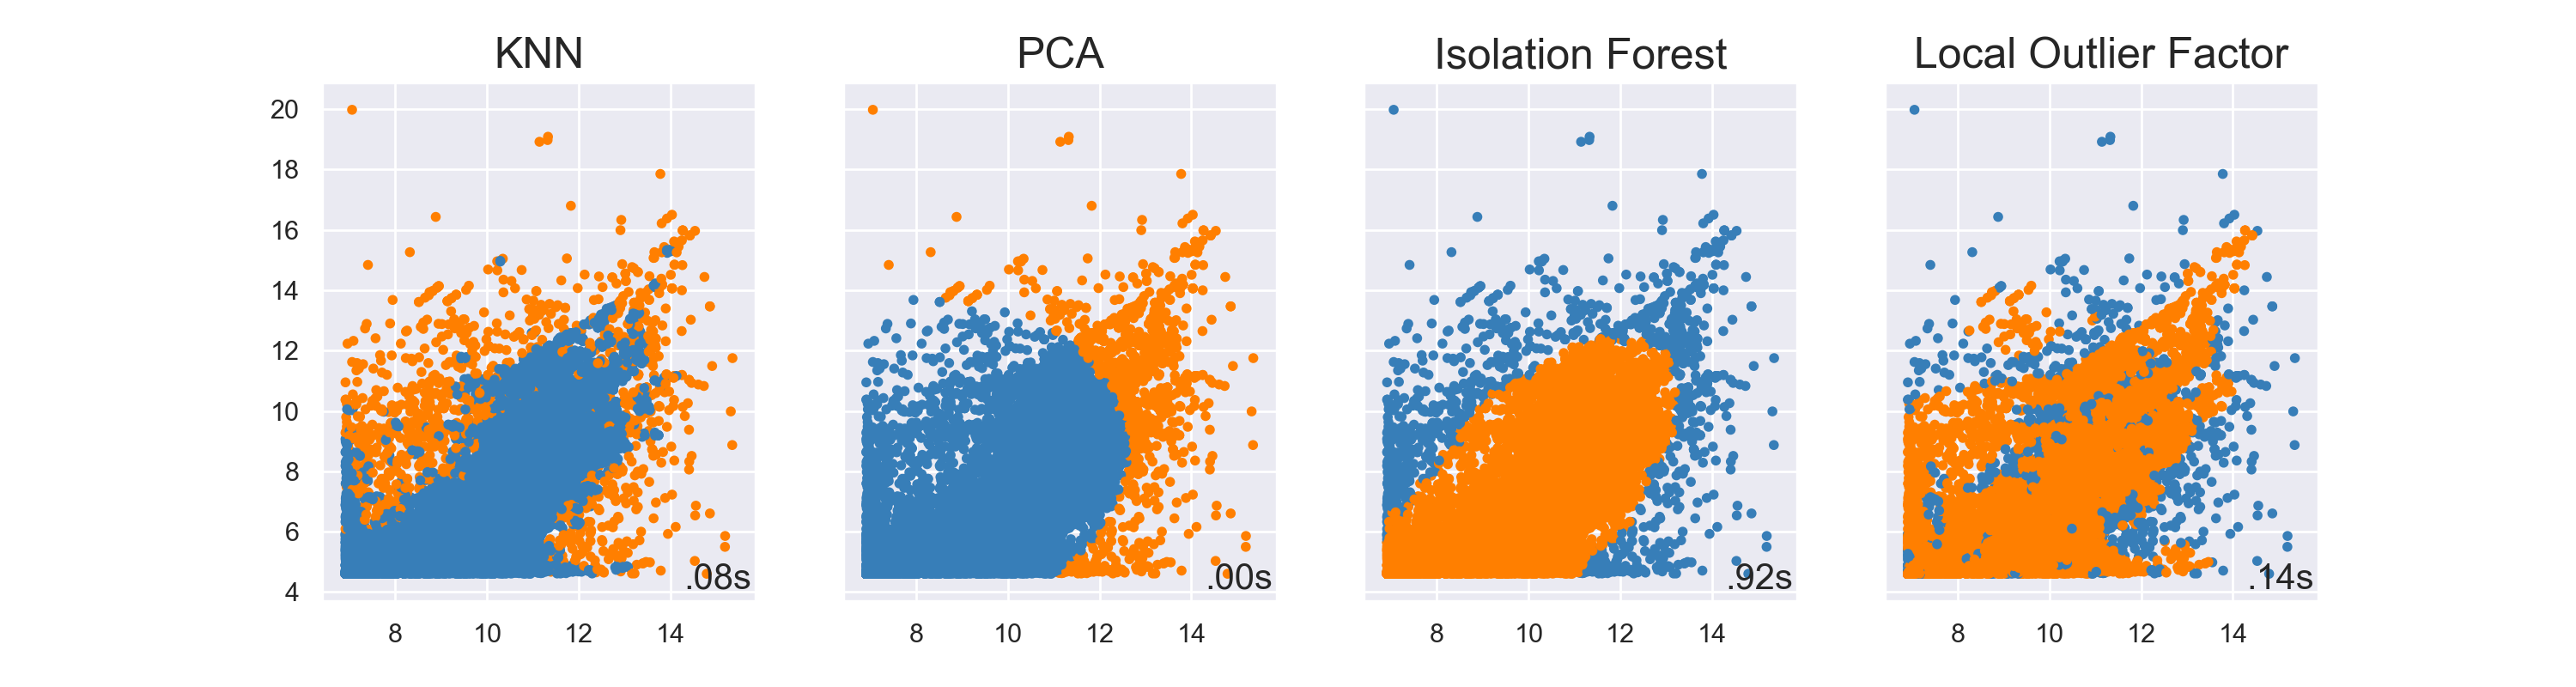
\includegraphics[width=1.06\textwidth]{ADOA/Images/sale_algo.png}
    \caption{Les transactions frauduleuses détectées comme des valeurs aberrantes par PCA, KNN, Isolation Forest and LOF.}%\hrule
    \label{fig_sal2}
\end{figure*}

%\afterpage{\FloatBarrier}

\afterpage{\FloatBarrier}